%\documentclass[10pt,handout]{beamer}
\documentclass[10pt]{beamer}
\usepackage[english]{babel} % Anpassa efter svenska. Ger svensk logga.
\usepackage[utf8]{inputenc} % Anpassa efter linux
\usepackage{graphicx}
\usetheme{Uppsala}
%\usecolortheme{UU} % Anpassa efter UU:s frger och logga
%\hypersetup{pdfpagemode=FullScreen} % Adobe Reader ska ppna fullskrm
\setbeamertemplate{itemize items}[circle]

% \usepackage{beamerthemesplit}
\usepackage{amsmath}
\usepackage{amssymb}
% \usepackage{graphics}
% \usepackage{graphicx}
% \usepackage{epsfig}
% \usepackage[latin1]{inputenc}
 \usepackage{color}
% \usepackage{fancybox}
% \usepackage{psfrag}
% \usepackage[english]{babel}
 \setbeamertemplate{footline}{\hfill\insertframenumber/\inserttotalframenumber}


%library(tinytex)
%tlmgr_install('csquotes')
\usepackage{csquotes}

%\usepackage{bm}
%\usepackage{natbib}
\newcommand{\bfm}[1]   {\mbox{\boldmath{${#1}$}}}
\newcommand{\Prob}   {\mbox{\textnormal{P}}}
\def\eqd{\,{\buildrel d \over =}\,}
\DeclareMathOperator{\E}{\mathbb{E}}

%%%%%%%%%%%%%%%%%%%%%%%%%%%%%%%%%%%%%%%%%%%%%%%%%%%%%%%%%%%%%%%%%%

\setlength{\parskip}{3mm}
\title[]{{\color{black}Machine learning, big data and artificial intelligence -- Block 7}}
\author[]{M{\aa}ns Magnusson\\Department of Statistics, Uppsala University}
\date{HT 2021}


\begin{document}

\frame{\titlepage
% \thispagestyle{empty}
}

%%%%%%%%%%%%%%%%%%%%%%%%%%%%%%%%%%%%%%%%%%%%%%%%%%%%%%%%%%%%%%%%%%


\begin{frame}{This week's lectures}
\begin{itemize}
\item Introduction to unsupervised learning
\item k-means
\item Mixture of Gaussians
\item Expectation-Maximization
\item Probabilistic PCA
\end{itemize}
\end{frame}


%%%%%%%%%%%%%%%%%%%%%%%%%%%%%%%%%%%%%%%%%%%%%%%%%%%%%%%%%%%%%%%%%%



\section{Previous assignments}

\begin{frame}{Practicalities}

\begin{itemize}
\item Remember the project proposition deadline the 15th of December
\item An additional guest lecture in January on fairness in AI and law (Holli Sargeant, Cambride University)
\end{itemize}

\end{frame}

\begin{frame}{Assignment 4}

\begin{itemize}
\item Not much
\end{itemize}

\end{frame}

\begin{frame}{Assignment 5: Evaluation}

\begin{itemize}
\item More variation
\item More example code
\item Would have liked to play around with BERT
\item Still not superclear what is the weights in the RNN: Keras confusion
\end{itemize}

\end{frame}

\begin{frame}{Recurrent Neural Networks}

\begin{align*}
a_t &= b + W h_{t-1} + U x_t \\
h_t &= \sigma_1(a_t) \\
o_t &= c + V h_{t} \\
\hat{y}_t & = \sigma_{\text{output}}(o_t) = \text{softmax}(o_t)
\end{align*}

Think of $h_t$ as the "state" at timepoint $t$

The embedding is $X$.

\end{frame}


\section{Introuction to unsupervised learning}

\begin{frame}{Supervised and Unsupervised learning}

\begin{figure}[h]
\centering
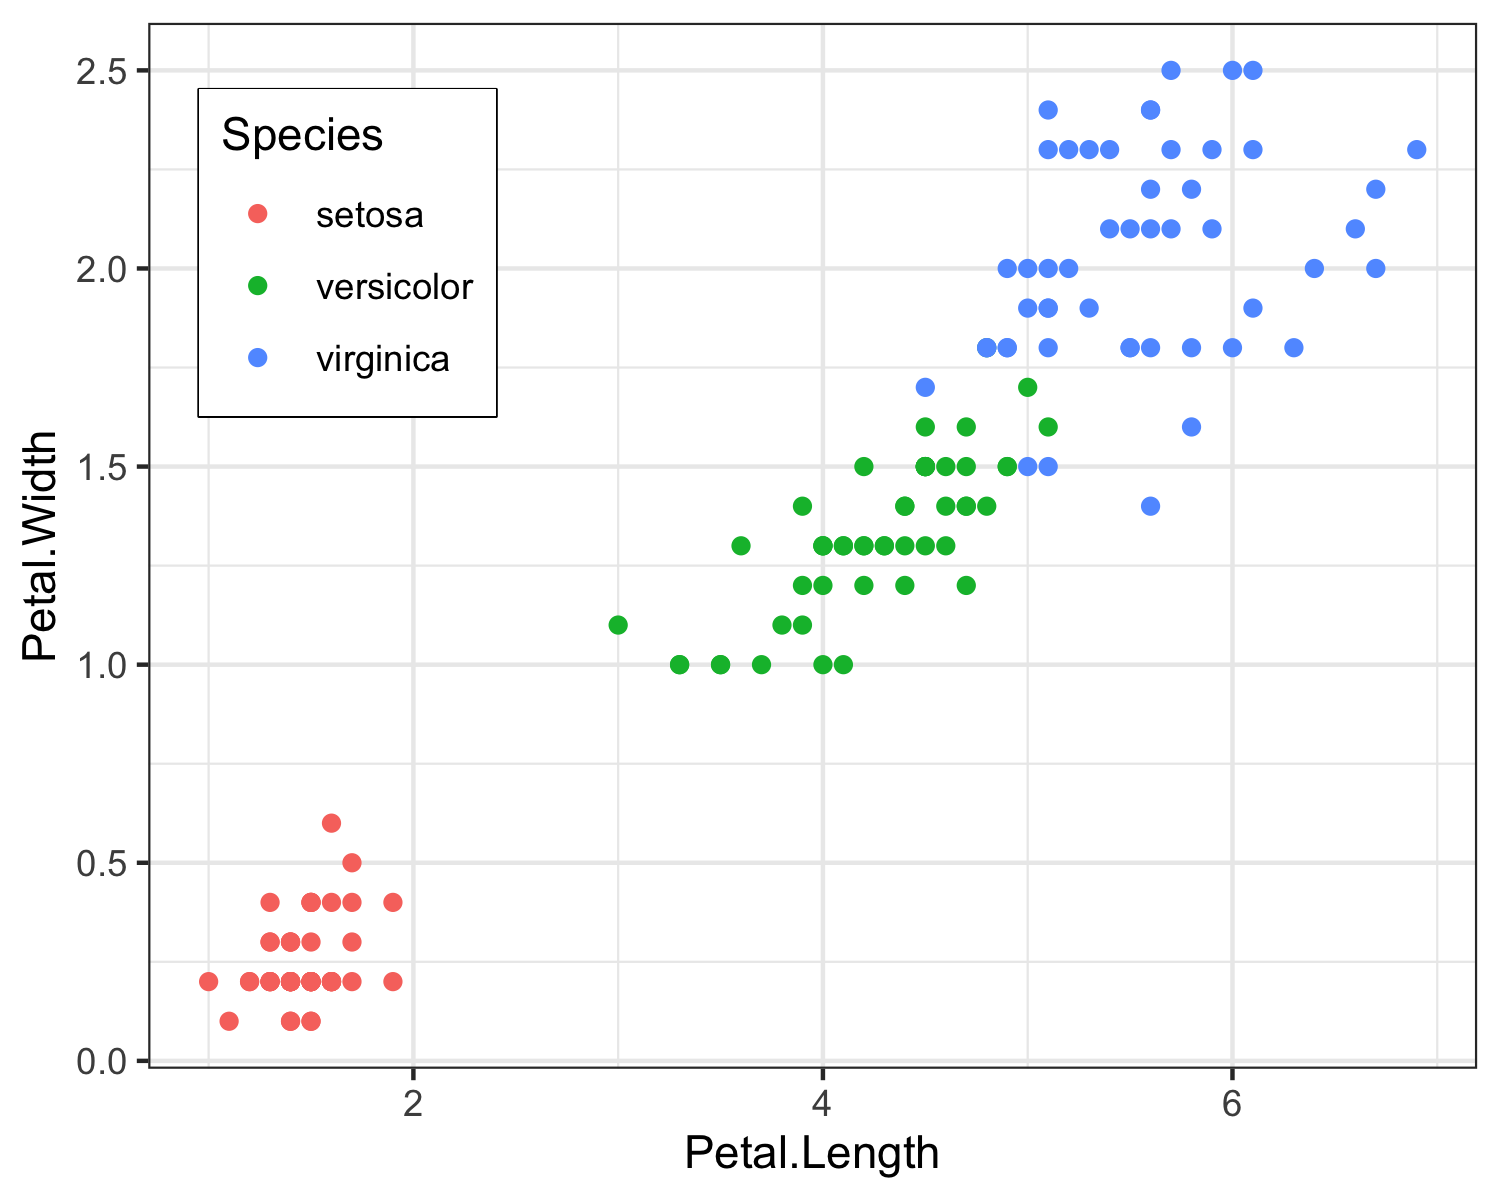
\includegraphics[width=0.9\textwidth]{fig/iris_supervised.png}
\caption{The Supervised Problem}
\end{figure}

\end{frame}

\begin{frame}{Supervised and Unsupervised learning}

\begin{figure}[h]
\centering
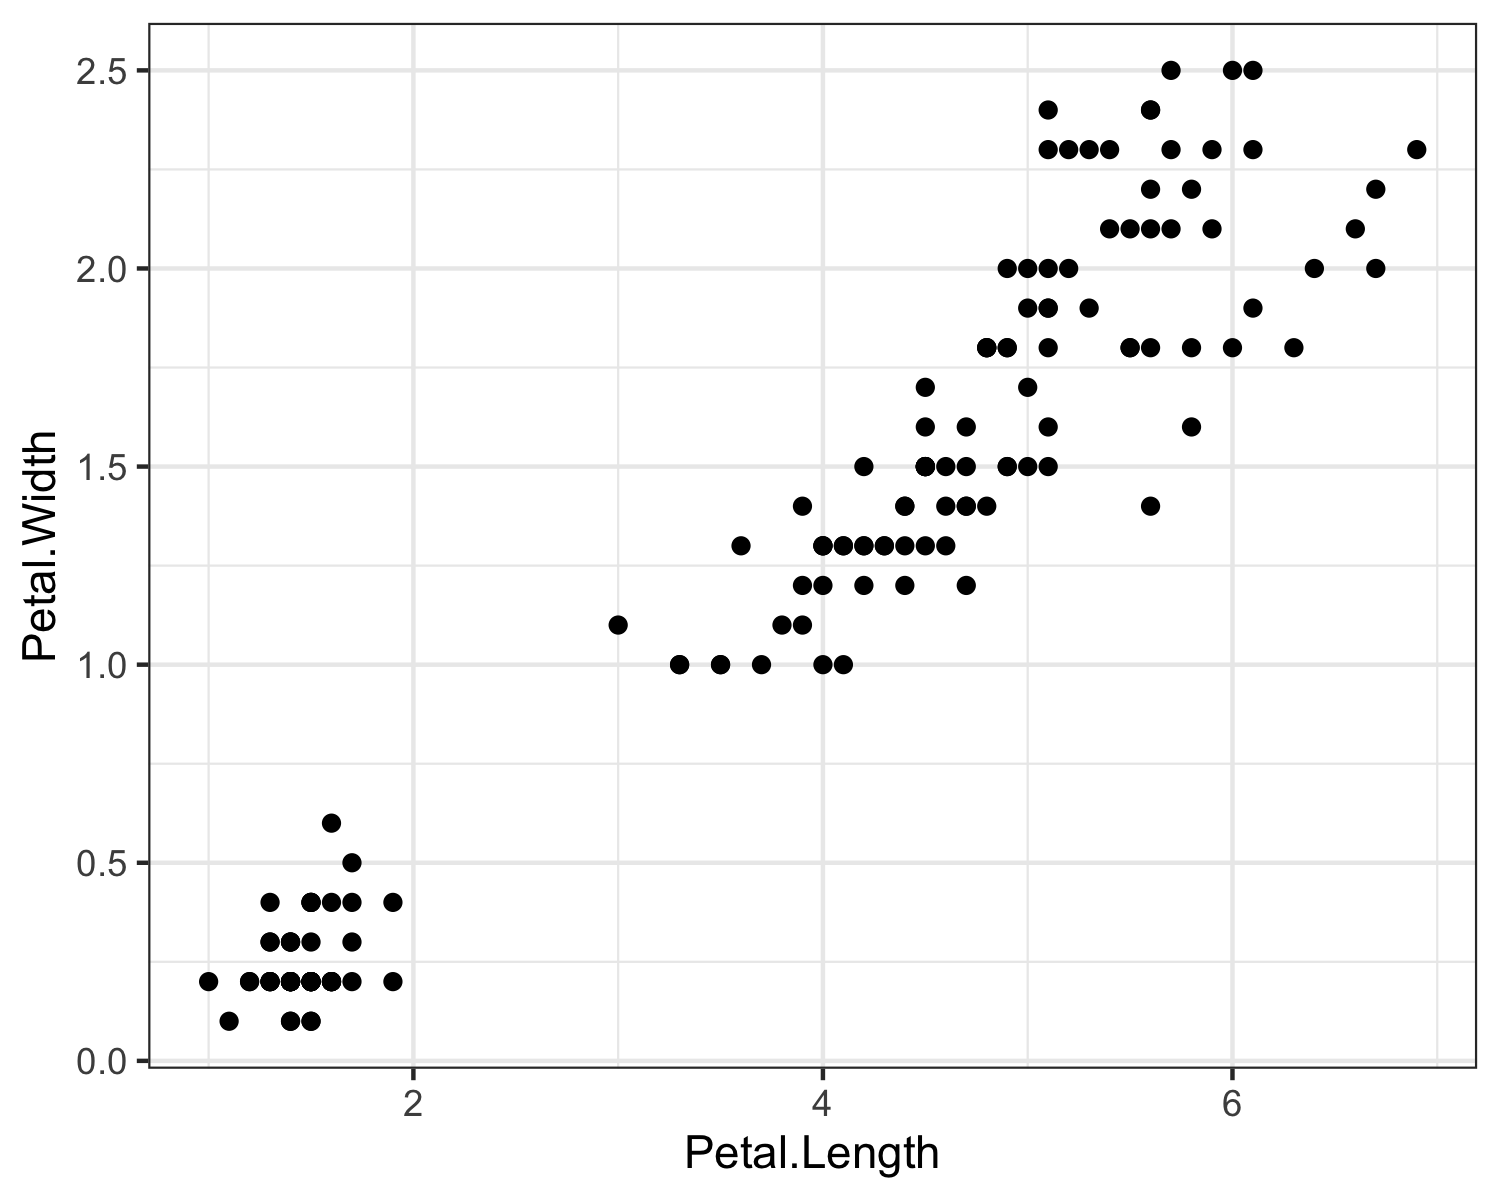
\includegraphics[width=0.9\textwidth]{fig/iris_unsupervised.png}
\caption{The Unsupervised Problem}
\end{figure}

\end{frame}


\begin{frame}{Supervised and Unsupervised learning}

In {\color{uured} supervised} learning:
\begin{itemize}
\item We have \emph{training} data
\[
\mathbf{d} = \{(y_i, \mathbf{x}_i), i = 1, ..., n\} \,.
\]
\item We train a model $p(y|x)$ to {\color{uured} predict} $y$
\item We only care about the loss function during training
\end{itemize}
\pause
In {\color{uured} unsupervised}  learning:
\begin{itemize}
\item We have \emph{training} data
\[
\mathbf{d} = \{(\mathbf{x}_i), i = 1, ..., n\} \,.
\]
\item We train a model $p(x)$ to {\color{uured} explain/model} $x$
\item Our loss function (or model) can be the goal
\end{itemize}
\end{frame}


\begin{frame}{Unsupervised learning}

{\color{uured} Goal}: Build a good (probabilistic) model $p(x)$ for $x$

\pause

Other names for $p(x)$:
\begin{itemize}
\item {\color{uured} Data} model\\ $p(x)$ is our \emph{data} generating mechanism
\item {\color{uured} Generative} model\\ We can \emph{generate} samples from $p(x)$.
\end{itemize}
\pause
Common use cases for unsupervised learning:
\begin{itemize}
\item Generate new observations from $p(x)$ % GAN/VAE
\item Study structure in large data % Topic models
\item Anomaly detection % Outbreak detection
\item Create representations for downstream tasks % Word embeddings
\end{itemize}

\end{frame}


\begin{frame}{The Learning Problem}

\begin{itemize}
\item {\color{uured} Goal}: A model that can "explain" the data well
\item Two main approaches:
\begin{itemize}
\item {\color{uured} Clustering}: Finding similar {\color{uured} observations} (rows)
\item {\color{uured} Dimensionality reduction}: Finding similar {\color{uured} variables} (columns)
\end{itemize}
\pause
\item Commonly, we use parametric probabilistic models\\ $p(x|\theta)$ where $\theta$ is unknown
\item {\color{uured} Learning problem}: Learn $\theta$ to explain the data as good as possible
\end{itemize}

\end{frame}


\begin{frame}{Example: Autoencoder}

\begin{figure}[h]
\centering
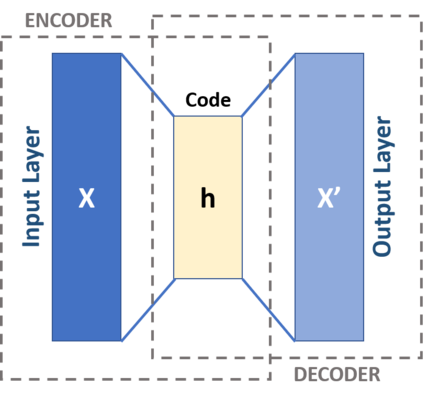
\includegraphics[width=0.8\textwidth]{fig/440px-Autoencoder_schema.png}
\caption{A Neural Autoencoder (Wikipedia)}
\end{figure}

\end{frame}

\begin{frame}{Loss functions and evaluation}
\begin{itemize}
\item Autoencoder uses the difference between the original and reconstructed output
\[
L(x) = (d(e(h|x)|h) - x)^2\,,
\]
where $d(x|h)$ is the decoder and $e(h|x)$ is the encoder.\pause
\item In probabilistic models we can use the log-likelihood ($\mathcal{L}$) \\ Sometimes called {\color{uured} perplexity} or {\color{uured} surprise}.
\begin{itemize}
\item {\color{uured} High} $\mathcal{L}$: The observation is {\color{uured} well} explained by the model
\item {\color{uured} Low} $\mathcal{L}$: The observation is {\color{uured} badly} explained by the model
\end{itemize}
\item Common approach: Evaluate log-likelihood on a held-out set
\end{itemize}

\end{frame}



\begin{frame}{Example: Bivariate Gaussian model}

\begin{figure}[h]
\centering
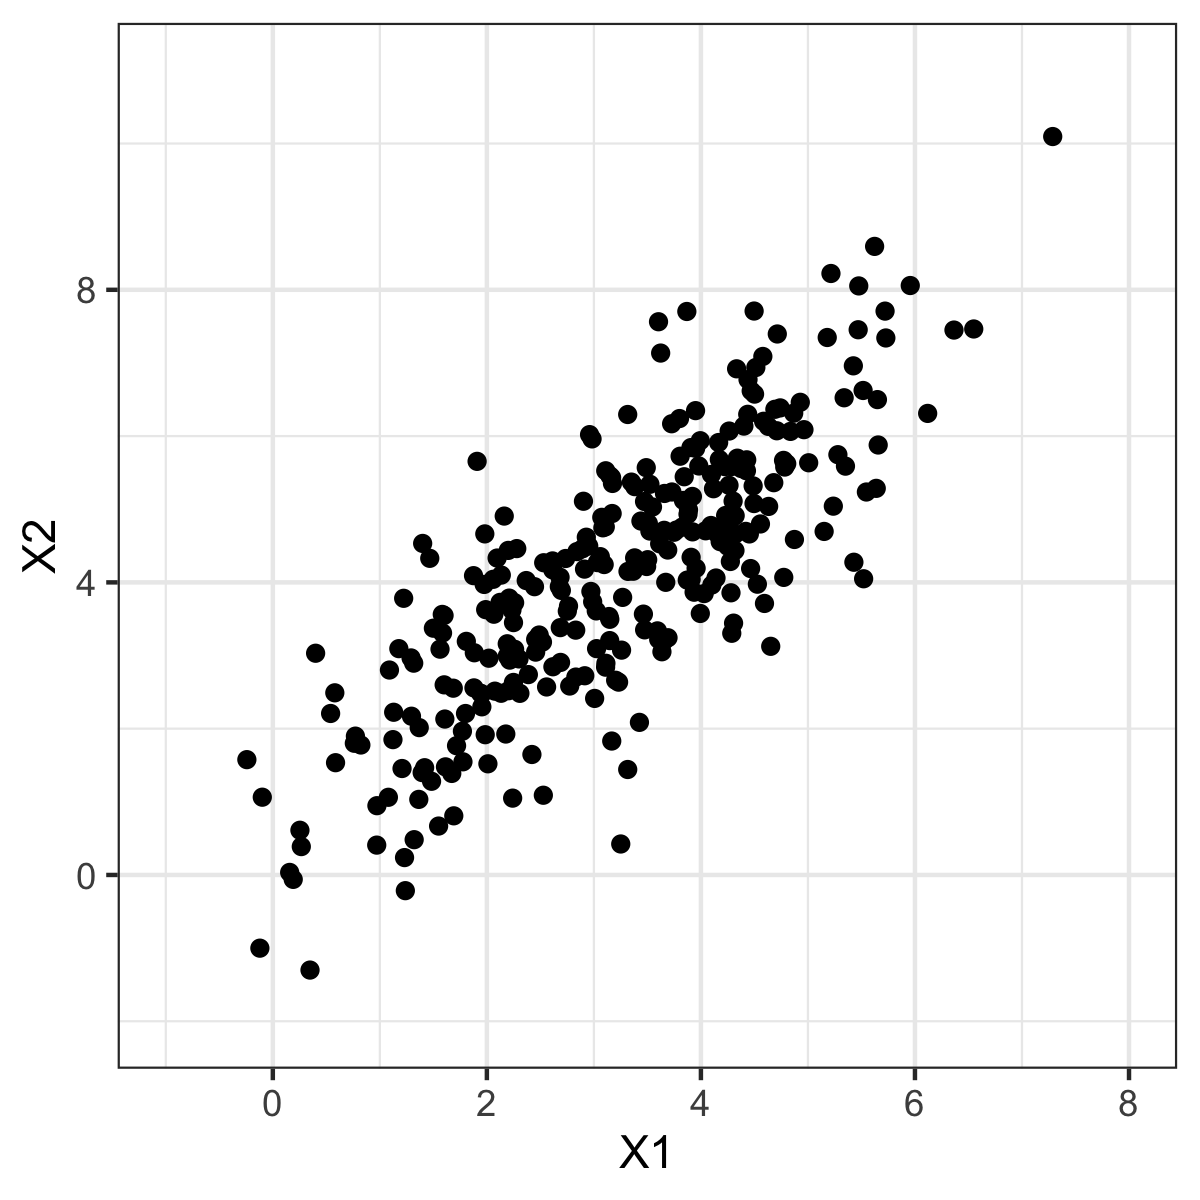
\includegraphics[width=0.9\textwidth]{fig/bi_data.png}
\caption{A Neural Autoencoder (Wikipedia)}
\end{figure}

\end{frame}

\begin{frame}{Example: Bivariate Gaussian model}

We assume a Multivariate Gaussian model and estimate $\mu,\Sigma$ from data.

\[
\hat{\mu} = [3.19, 4.11]
\]

\[
\hat{\Sigma} = \begin{bmatrix} 1.95 & 2.05\\ 2.05 & 3.36 \end{bmatrix}
\]

We can now generate new data from MVN($\hat{\mu},\hat{\Sigma}$).

\end{frame}

\begin{frame}{Example: Bivariate Gaussian model}

\begin{figure}[h]
\centering
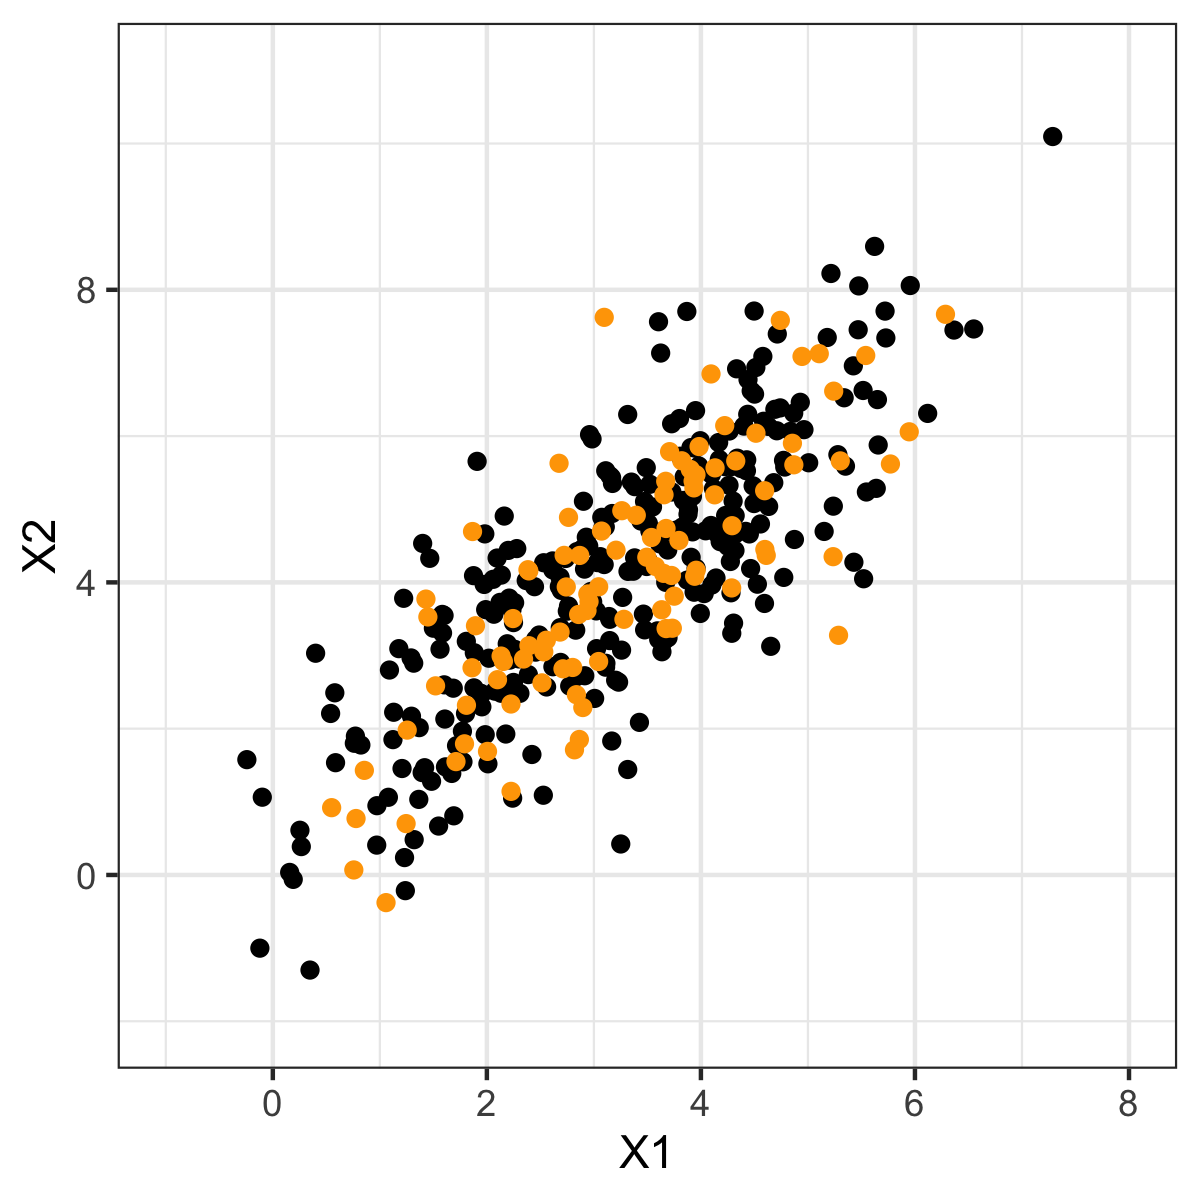
\includegraphics[width=0.9\textwidth]{fig/bi_model.png}
\caption{A Neural Autoencoder (Wikipedia)}
\end{figure}

\end{frame}




\subsection{Latent variables}

\begin{frame}{Latent variables}
\begin{itemize}
\item An {\color{uured} unobserved} or {\color{uured} hidden} variable or "factor"\pause
\item A parameter specific to some or a few observations or features\pause
\item Often these latent variables can be of interest
\end{itemize}

\end{frame}

\begin{frame}{Example: Hidden Markov Model}

\begin{figure}[h]
\centering
\includegraphics[width=0.9\textwidth]{fig/hmm.png}
\caption{A Hidden Markov Model (Wikipedia). Note that $x$ is unobserved and $y$ is observed.}
\end{figure}

\end{frame}

\begin{frame}{Example: Factor Analysis}

\begin{figure}[h]
\centering
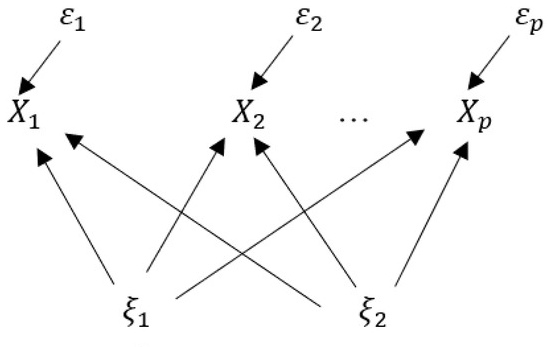
\includegraphics[width=0.9\textwidth]{fig/FM.png}
\caption{A Factor Analysis Model (Eshima, Tabata and Borroni, 2018, edited).}
\end{figure}

\end{frame}



\section{Clustering}


\begin{frame}{Clustering}
\begin{itemize}
\item Separate observations $x_i$ into {\color{uured} groups} or {\color{uured} segments}\pause
\item What is a cluster "is" depends on the {\color{uured} model/(dis)similarity}.
\item (Dis)similarity:
\[
D(x_i, x_j) = \sum_{k = 1}^P d_k(x_{i,k}, x_{j,k})
\]
\item A common dissimilarity is the squared distance
\[
d_k(x_{i,k}, x_{j,k}) = (x_{i,k} - x_{j,k})^2
\]
\pause
\item Clustering can be divided into:
\begin{itemize}
\item {\color{uured} Hard} clustering%: An observation belong only to one cluster
\item {\color{uured} Soft} clustering%: An observation has a probability of belonging to all clusters (but it might be 0)
\end{itemize}
\pause
\item Clustering can also be divided into:
\begin{itemize}
\item {\color{uured} Hiearchical} clustering
\item {\color{uured} Flat} clustering
\end{itemize}
\pause
\item There is a ton of different algorithms and methods...
\end{itemize}

\end{frame}

\begin{frame}{k-means}
\begin{itemize}
\item Popular in practice and a classic in unsupervised machine learning\pause
\item Hard, flat clustering
\item Simple and effective\pause
\item {\color{uured} Model}: $x_i$ is close to one of $m_1,...,m_K$ vectors
\item {\color{uured} Loss function}:
\[
l_\mathbf{m} (x) = \min_\mathbf{m} (x_i - m_k)^2
\]
\pause
\item {\color{uured} Hyperparameter}: $K$ (the number of clusters)
\item {\color{uured} Parameters}:  $\mathbf{m}$ (a $K \times P$ matrix).
\pause
\item A {\color{uured} difficult} problem: $K^n$ possibilities
\end{itemize}

\end{frame}


\begin{frame}{k-means algorithm}

\begin{figure}[h]
\centering
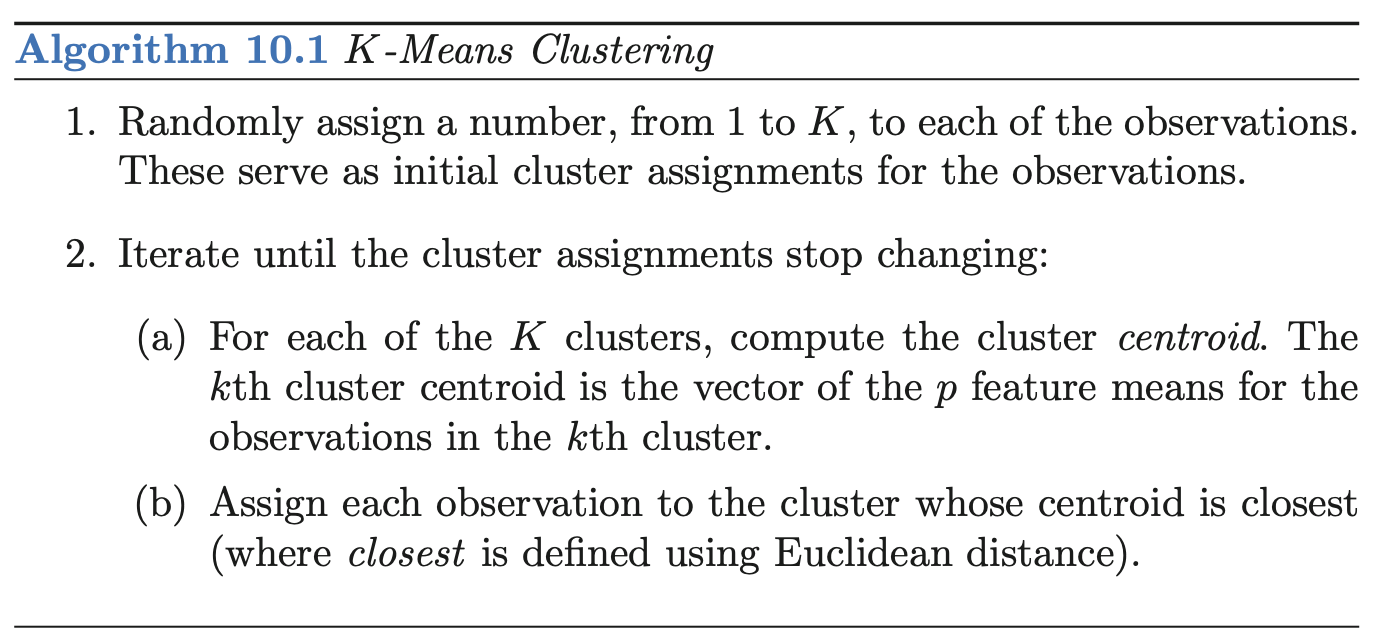
\includegraphics[width=0.9\textwidth]{fig/algo_10_1_kmeans.png}
\caption{The k-means cluster algorithm (Garreth et al, 2013, Alg. 10.1).}
\end{figure}


\end{frame}



\begin{frame}{k-means clustering}

\begin{figure}[h]
\centering
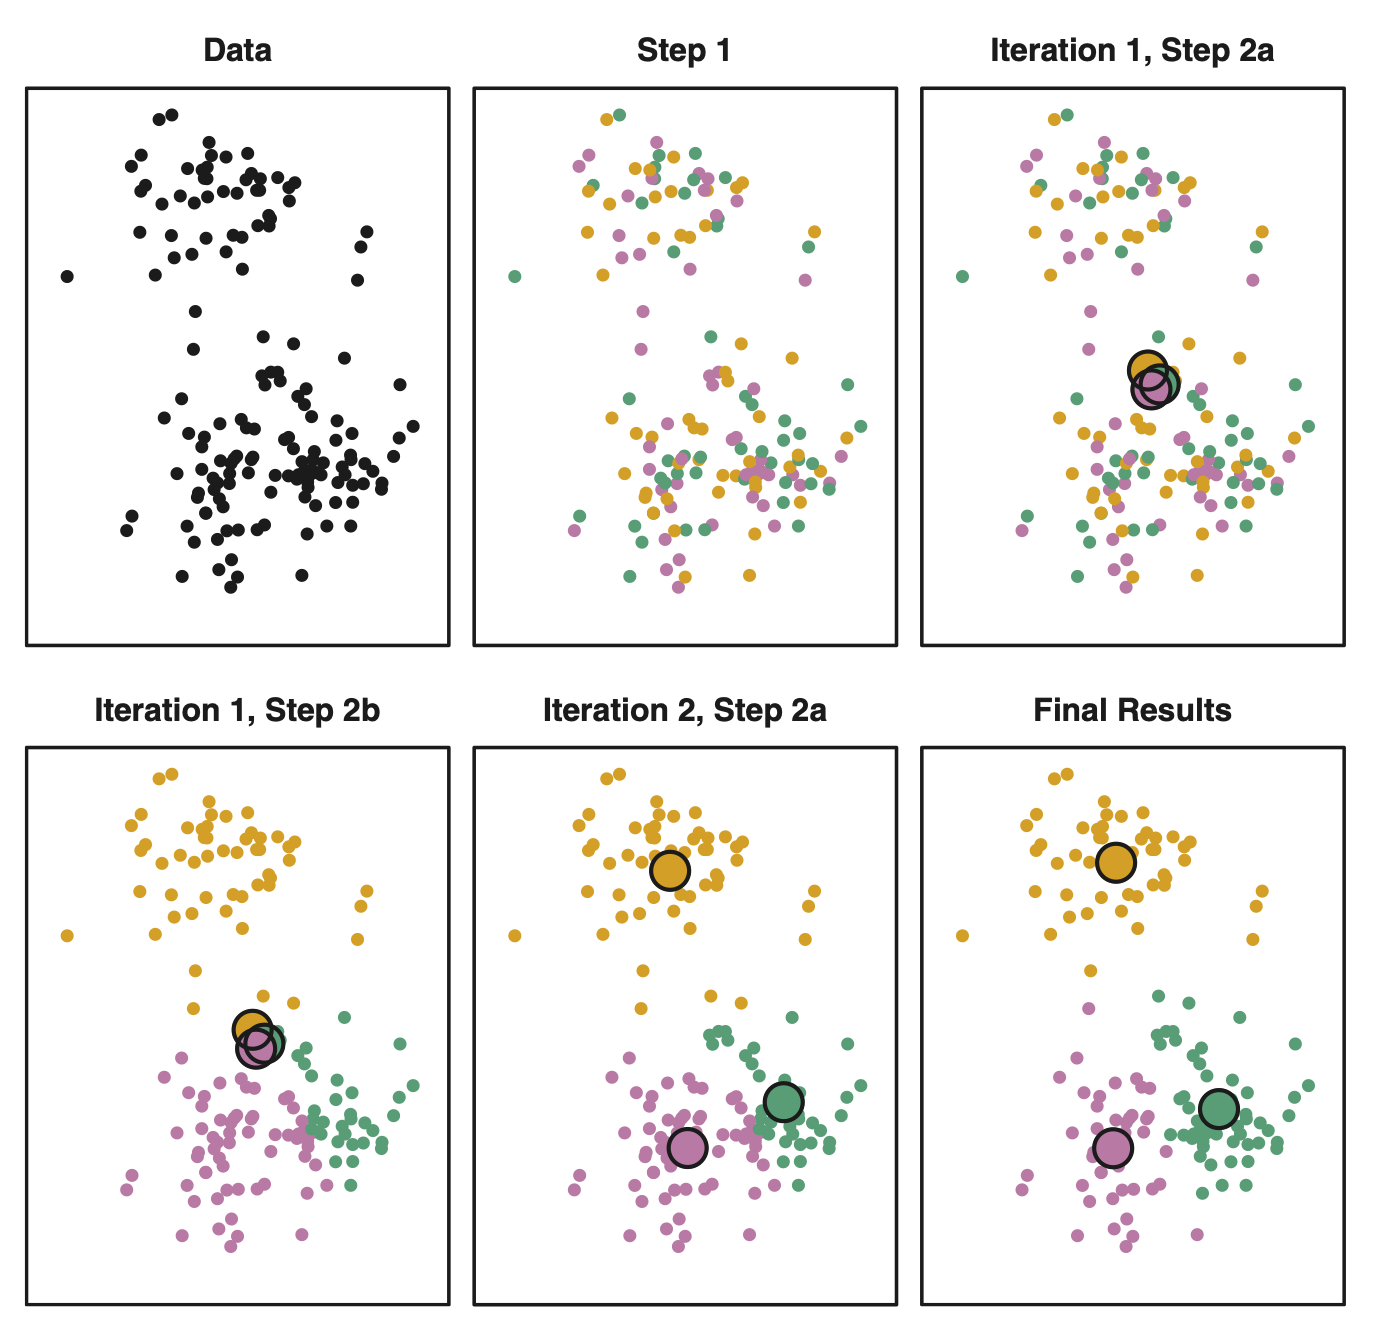
\includegraphics[width=0.75\textwidth]{fig/fig_10_6_kmeans_algo.png}
\caption{The k-means cluser algorithm (Garreth et al, 2013, Fig. 10.6).}
\end{figure}

\end{frame}


\begin{frame}{k-means clustering}

\begin{itemize}
\item k-means finds {\color{uured} local modes}
\item Re-run algorithm with many {\color{uured} different starting values}
\item Choose the best by the best loss
\pause
\item There exists many developments
\begin{itemize}
\item scaling to large data
\item generalized loss
\item approaches to find a good $K$
\end{itemize}
\end{itemize}
\end{frame}


\begin{frame}{k-means clustering}

\begin{figure}[h]
\centering
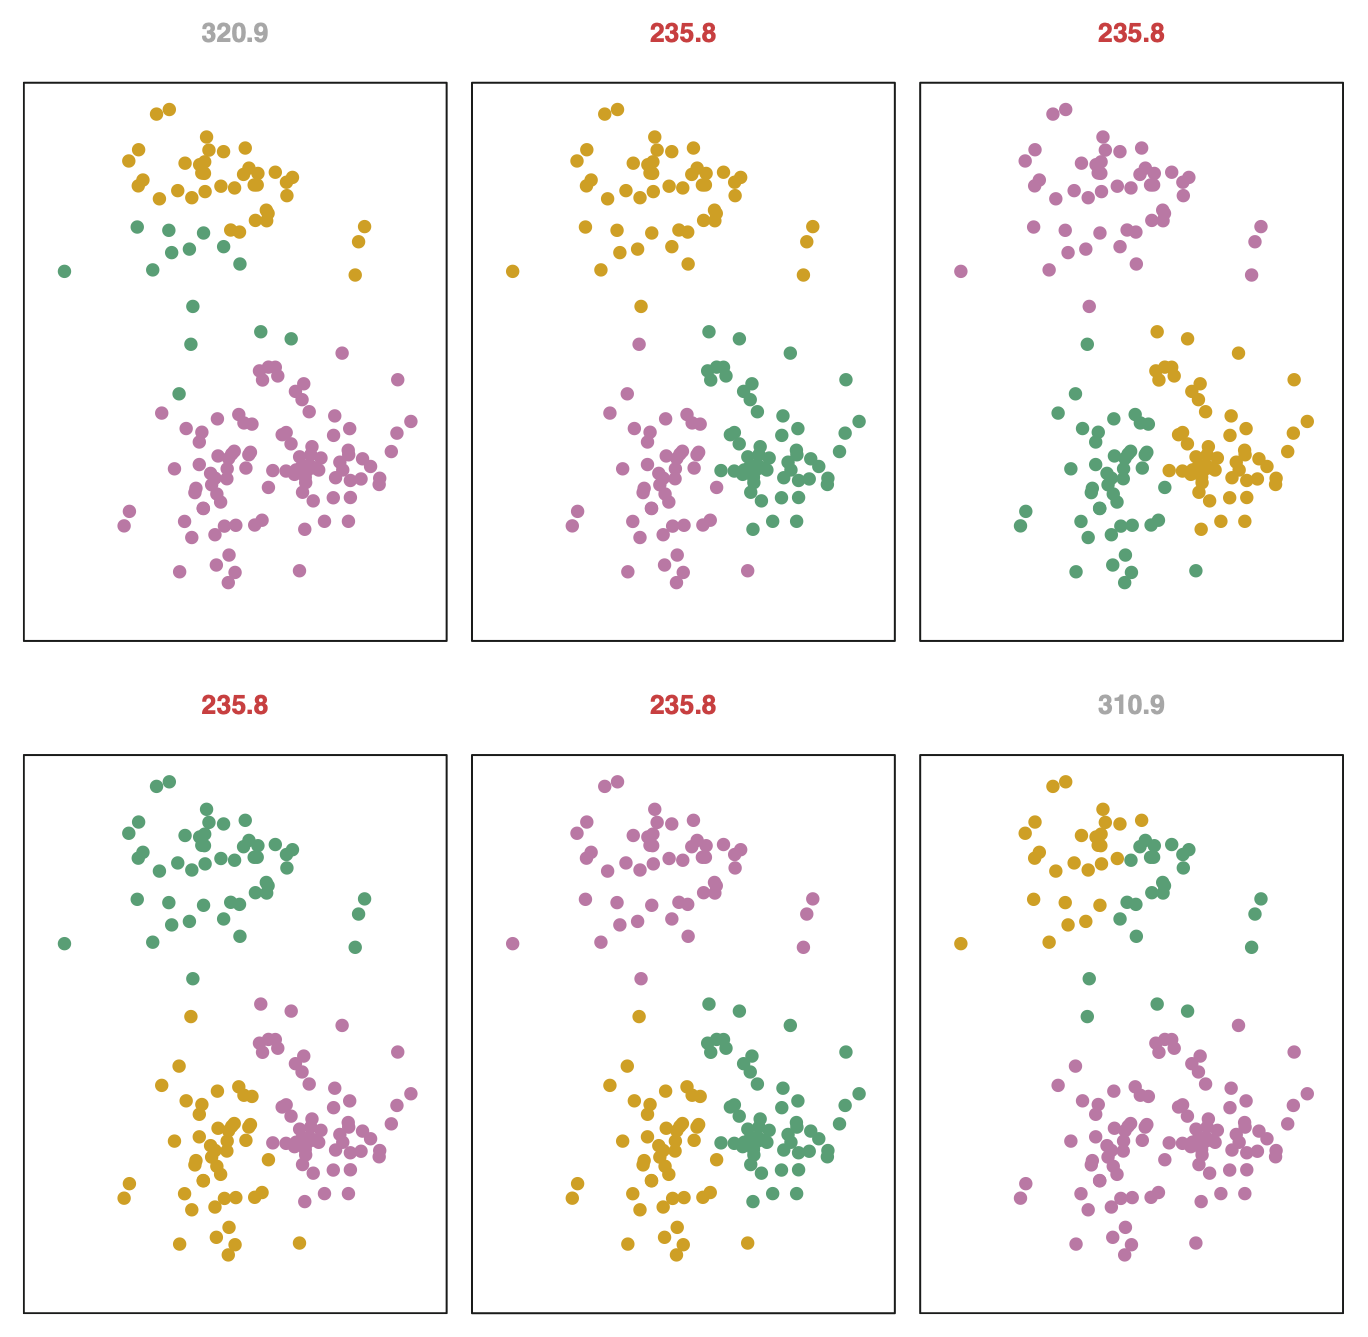
\includegraphics[width=0.75\textwidth]{fig/fig_10_7_kmeans_local_modes.png}
\caption{The k-means cluser algorithm (Garreth et al, 2013, Fig. 10.7).}
\end{figure}

\end{frame}


\section{Mixture models}

\begin{frame}{Problems with k-means}

\begin{itemize}
\item Clusters might
\begin{itemize}
\item overlap
\item have different forms
\end{itemize}
\end{itemize}

\begin{figure}[h]
\centering
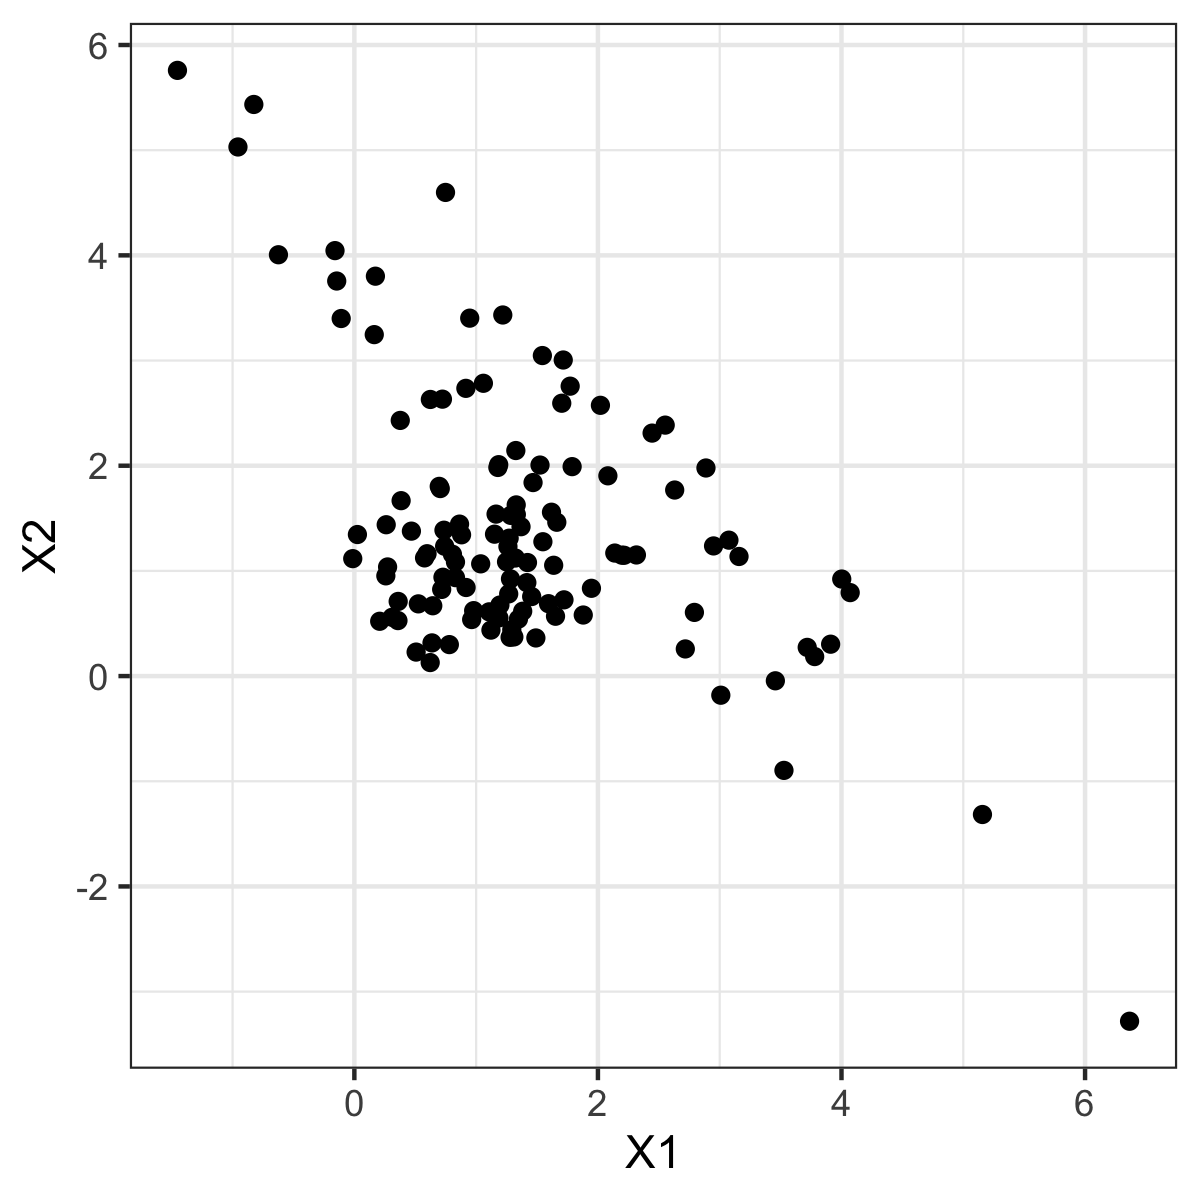
\includegraphics[width=0.4\textwidth]{fig/mix_models.png}
\caption{Two clusters with different shapes.}
\end{figure}

\pause
We can solve these problems using {\color{uured} probabilistic models}

\end{frame}

\begin{frame}{Finite Mixture Models}

% TODO: Derive the MM as a compound probability distribution.
The {\color{uured} finite mixture model} can be expressed as:

\[
y_i = \sum_{k=1}^K \pi_k \phi_k(\theta_k)\,,
\]

\begin{itemize}
\item The parts of a (finite) mixture model:
\begin{itemize}
\item The number of components: $K$\pause
\item The proportions of observation from component $k$: $\pi_k$\pause
\item The density of component $k$: $\phi_k$\pause
\item The parameters of component $k$: $\theta_k$
\end{itemize}
\end{itemize}

\end{frame}


\begin{frame}{Finite Mixture Models}

\begin{itemize}
\item Usually, we
\begin{itemize}
\item set $K$, and
\item use the same density for all $k$.
\end{itemize}
\pause
\item We can simulate data from the model as {\color{uured} compund probability distribution}:
\begin{enumerate}
\item Simulate cluster assignments for all $i$:
\[
z_i \sim \text{Categorical}(\pi)
\]
\item Generate $y_i$ conditioned on $z_i$:
\[
y_i \sim \phi_{z_i}(\theta_{z_i})
\]
\end{enumerate}
\item Cluster assignments $z_i$ are the {\color{uured} latent variables}
\end{itemize}

\end{frame}

\begin{frame}{Gaussian Mixture Models (GMM)}

\begin{itemize}
\item The (finite) Gaussian mixture model:
\[
y_i = \sum_{k=1}^K \pi_k \mathcal{N}(\mu_k, \Sigma_k)\,,
\]
where $\mu_k$ and $\Sigma_k$ depend on the dimensionality of $y_i$.\pause
\item GMM is a {\color{uured} universial approximator} of densities
% (Goodfellow et al. 2017, p. 67)
% A Gaussian mixture model is a universal approximator of densities, in the sense that any smooth density can be approximated with any specific nonzero amount of error by a Gaussian mixture model with enough components.
\end{itemize}

\end{frame}

\begin{frame}{Example: Simulate data from a GMM}

\begin{enumerate}
\item Generate cluster assignments:
\[
z_i \sim \text{Categorical}(\pi = [0.4, 0.6])
\]
\item Generate observation conditioned on cluster assignment:
\[
y_i \sim \mathcal{N}(\mu_k, \Sigma_k)\,,
\]
where
\[
\mu_1 = [2, 2]\,, \mu_2 = [1, 1]\, \text{and}
\]

\[
\Sigma_1 = \begin{bmatrix} 3 & -2.7\\ -2.7 & 3 \end{bmatrix}\,,\Sigma_2 = \begin{bmatrix} 0.2 & 0\\ 0 & 0.2 \end{bmatrix}
\]

\end{enumerate}

\end{frame}


\begin{frame}{Simulated data from a GMM}

\begin{figure}[h]
\centering
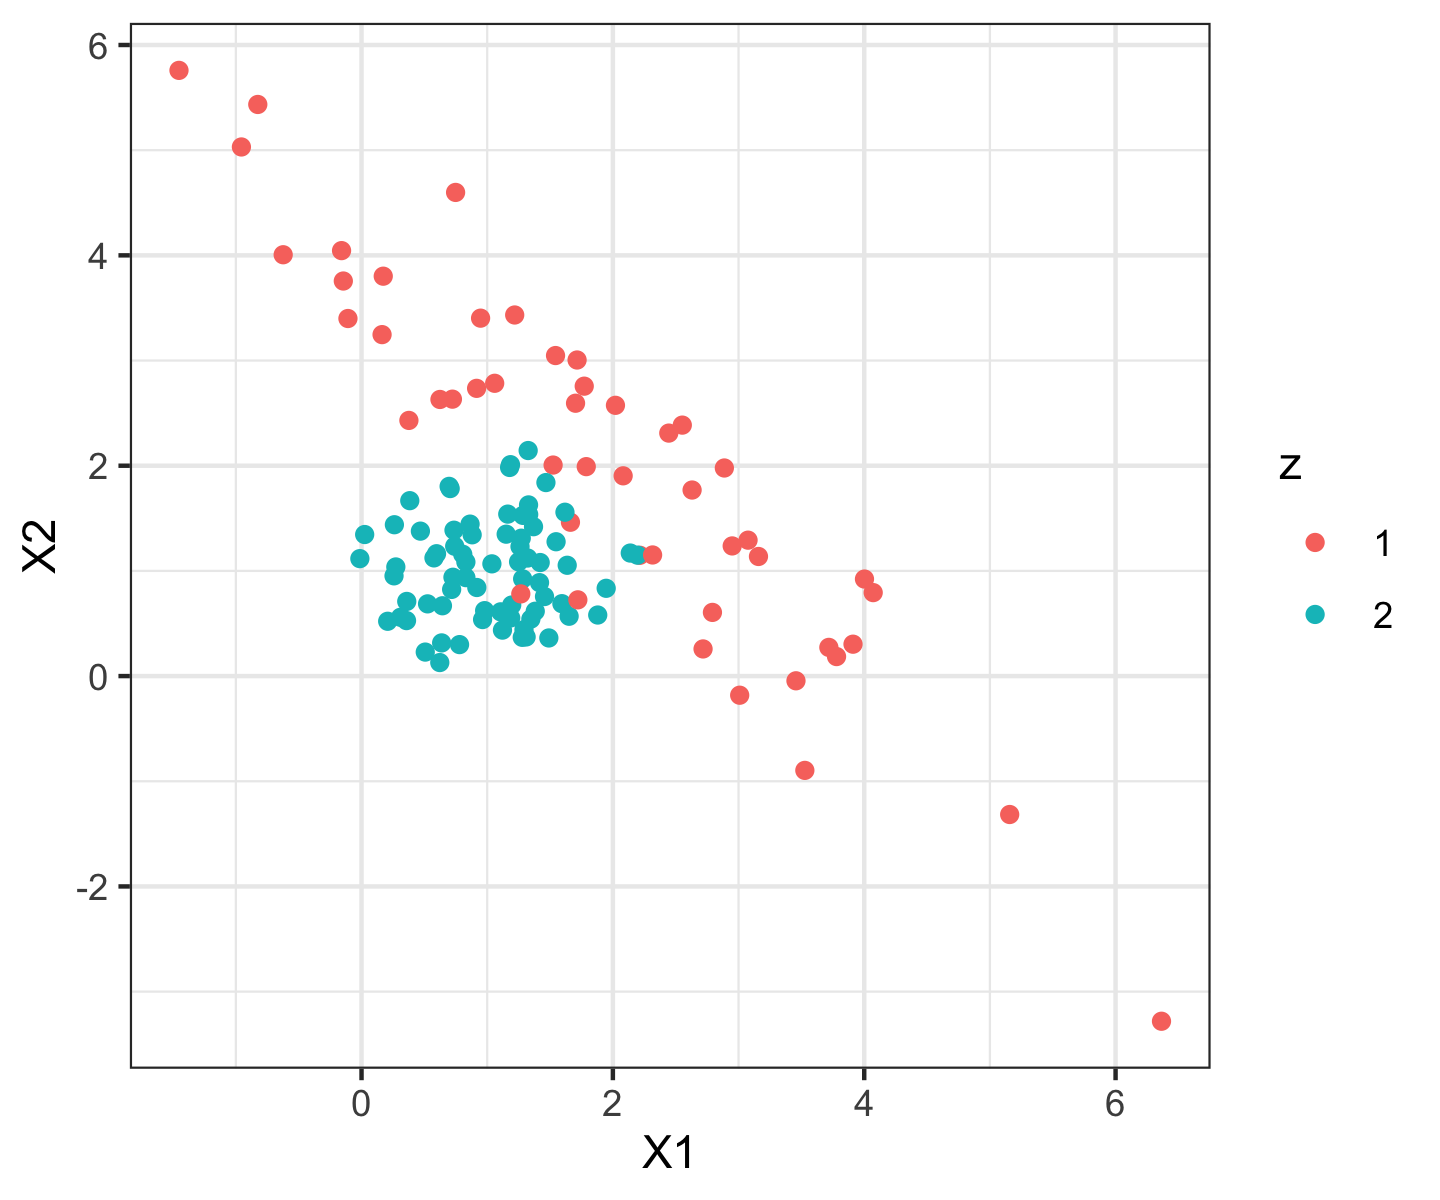
\includegraphics[width=0.5\textwidth]{fig/mix_models_z.png}
\caption{Simulated mixture data with the latent variable $z$.}
\end{figure}

\end{frame}


\begin{frame}{Mixtures of Multinomial distributions}

What {\color{uured} distribution} ($\phi$) should I use?\\
\pause
\vspace{2mm}
Depends on your {\color{uured} data} ($y$).
\pause

\[
y_i = \sum_{k=1}^K \pi_k \text{Multinomial}(\mathbf{p}_k)
\]

\begin{figure}[h]
\centering
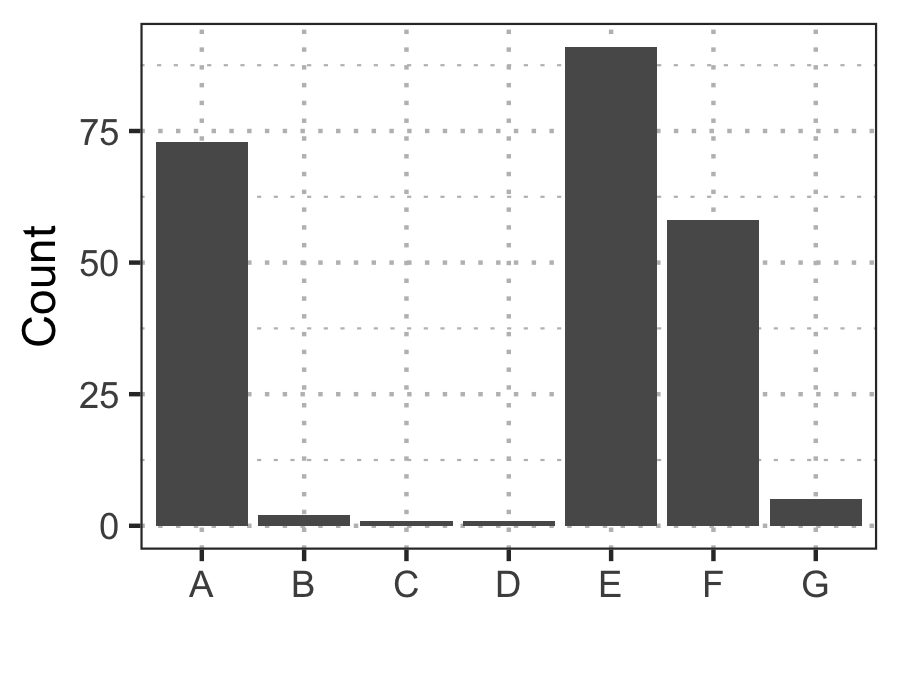
\includegraphics[width=0.25\textwidth]{fig/clu1.png}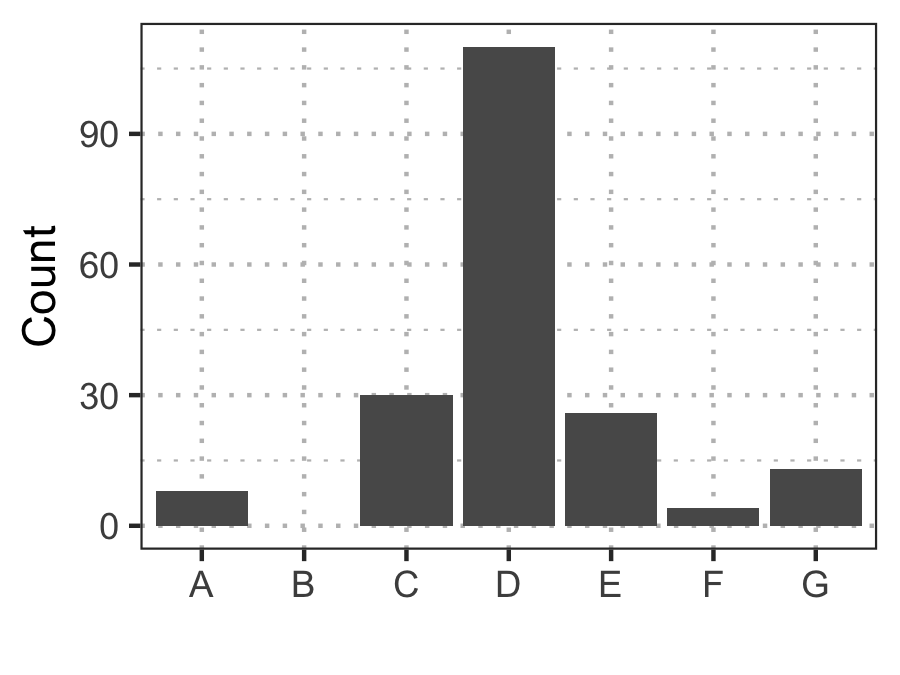
\includegraphics[width=0.25\textwidth]{fig/clu2.png}\\
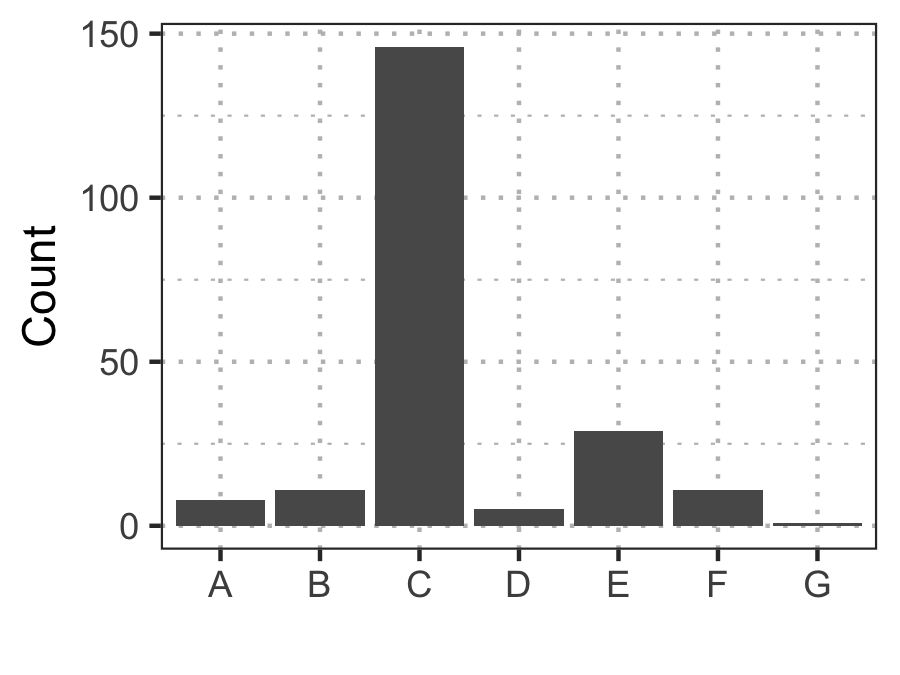
\includegraphics[width=0.25\textwidth]{fig/clu3.png}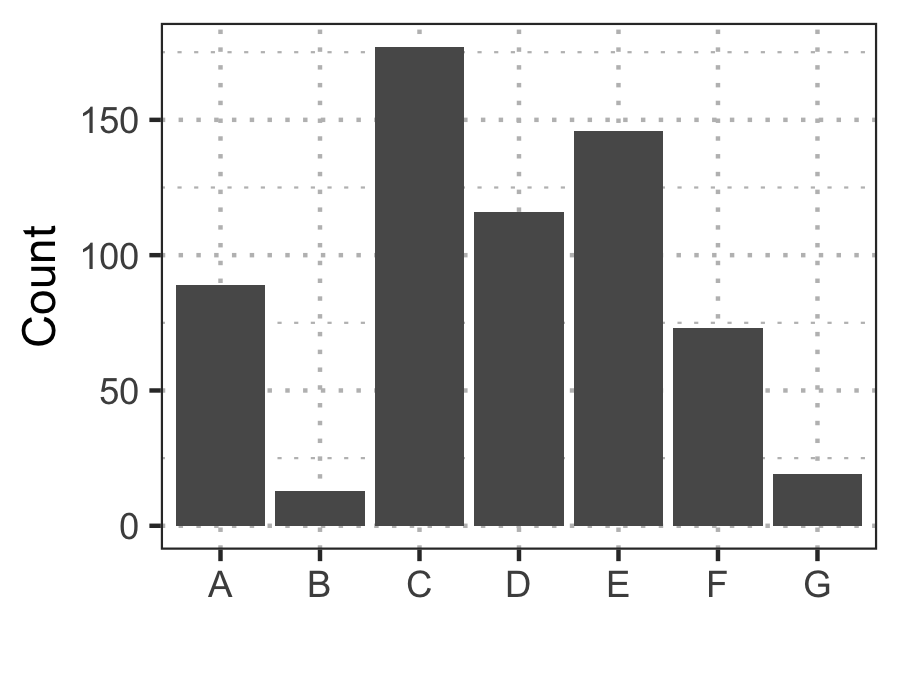
\includegraphics[width=0.25\textwidth]{fig/clu4.png}
\caption{Mixture of Multinomials.}
\end{figure}

\end{frame}


\section{Expectation Maximization}

\begin{frame}{Estimating Mixtures Models}

\begin{itemize}
\item We are interested in estimating $\theta_k$ and $\pi_k$ for the model
\[
y_i = \sum_{k=1}^K \pi_k \phi(\theta_k)\,,
\]
\item Hence we want to maximize the log-likelihood
\[
\mathcal{L}(\pi, \theta) = \sum^N_{i=1} \log \left( \sum_{k=1}^K \pi_k \phi(y_i|\theta_k)\right)
\]
\item This is difficult, although {\color{uured} if we only knew $\mathbf{z}$}...\pause
\begin{align*}
\mathcal{L}_{\text{full}}(\pi, \theta, \mathbf{z}) =& \sum^N_{i=1} \log \left( \sum_{k=1}^K I(z_i=k) \phi(y_i|\theta_k)\right) + \\
& \log(\pi_k^I(z_i=k))\\
=& \sum^N_{i=1} \sum_{k=1}^K I(z_i=k) \log \phi(y_i|\theta_k) + I(z_i=k) \log(\pi_k)
\end{align*}
\item So if we knew $\mathbf{z}$ it is essentially just maximizing $\mathcal{L}$ for each cluster separately.

\end{itemize}

\end{frame}


\begin{frame}{The Expectation}

\begin{itemize}
\item But, we dont know $\mathbf{z}$.\pause
\item Although, we could compute the {\color{uured} expected} cluster assignment
\[
\gamma_{i} = E_{z_i} (\mathcal{L}_{\text{full}}|\theta, y_i)\,.
\]
\item $\gamma_{i}$ can be seen as observation $i$s {\color{uured} weights} for each cluster
\item $\gamma_{i}$ is sometimes refered to as the {\color{uured} responsibility}.
\end{itemize}

\end{frame}


\begin{frame}{The Maximization}

\begin{itemize}
\item Now, given $\gamma$ we can (hopefully) easier maximize $\theta$.\pause
\item We maximize $\mathcal{L}_{\text{full}}$ given $\gamma$ and $y$.\pause
\item We usually choose $\psi$ so the maximization
\begin{itemize}
\item is a nice analytical expression.
\item end up with a weighted MLE.
\end{itemize}

\end{itemize}



\end{frame}

\begin{frame}{Example: EM for a Gaussian Mixture}

\begin{figure}[h]
\centering
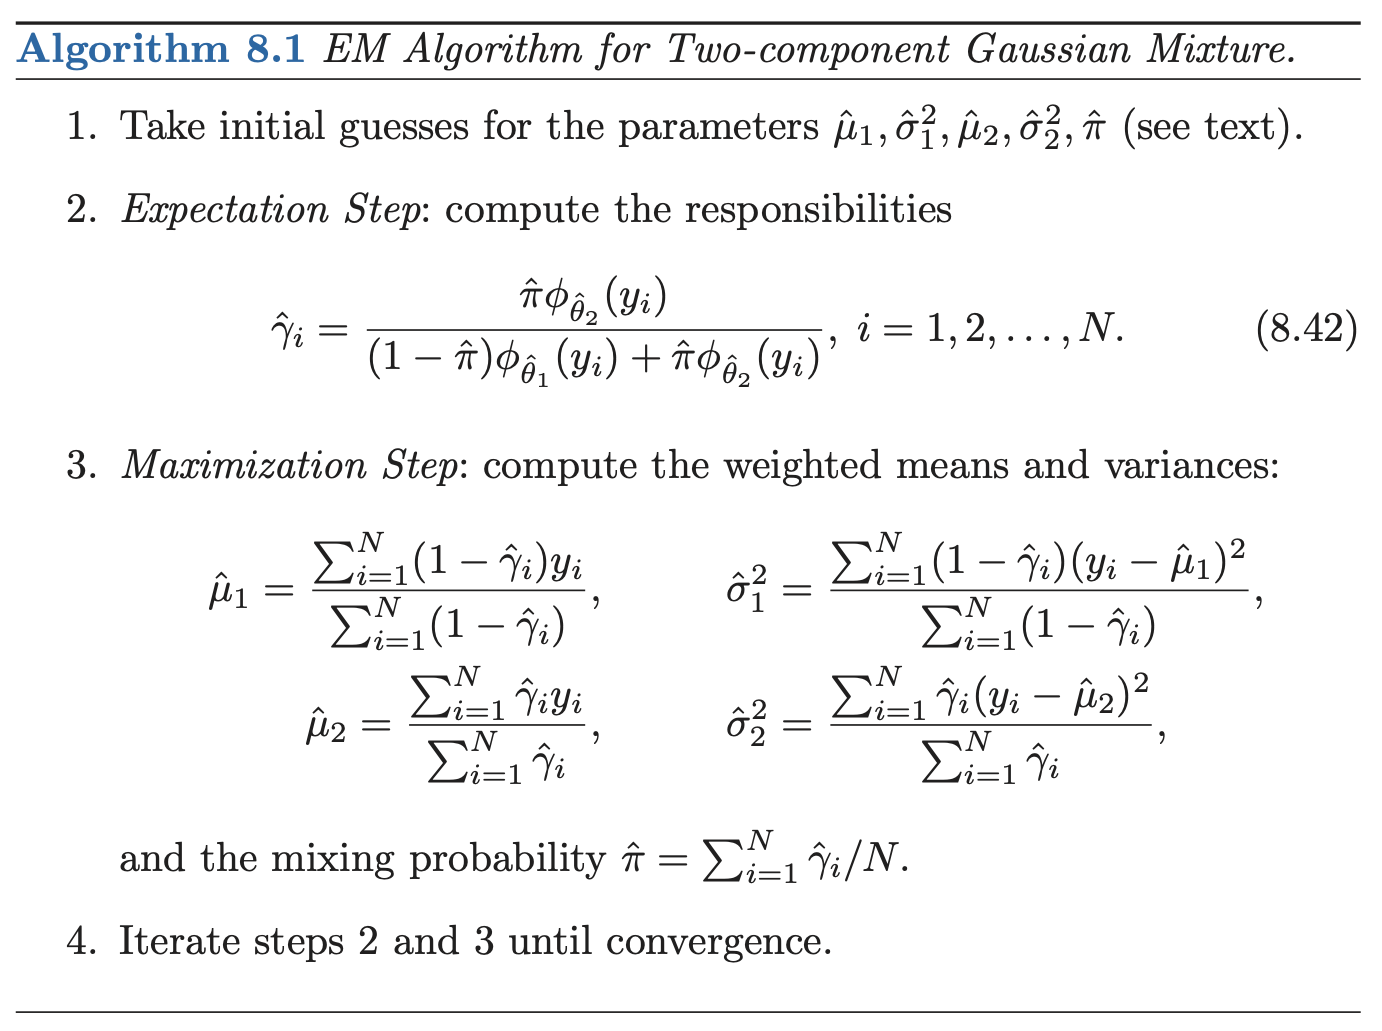
\includegraphics[width=0.9\textwidth]{fig/algo_8_1_em_gaussian.png}
\caption{The EM algorithm for a two component Gaussian mixture (Hastie et al 2008, Alg. 10.1)}
\end{figure}

\end{frame}

\begin{frame}{The EM algorithm}

\begin{itemize}
\item Properties of the EM algorithm:
\begin{itemize}
\item The EM-algorithm will converge to a {\color{uured} local mode}\pause
\item Each iteration will {\color{uured} always} increase the likelihood
\begin{itemize}
\item Can be proven straight-forward using Jensens inequality% (see optional assignment)
\end{itemize}
\pause
\item We can interpret the final $\gamma_i$ as the {\color{uured} expected cluster}\\
Hence, the EM algorithm is a {\color{uured} soft clustering} approach.
\end{itemize}
\item Expanding the likelihood with latent variables ($z$) is called {\color{uured} data augmentation}.
\\ \emph{Note!} Not the same as data augmentation in CNNs.
\end{itemize}

\end{frame}


\begin{frame}{Connections to other approaches}

\begin{itemize}
\item If we set $z_i = \text{argmax}(\gamma_i)$: {\color{uured} k-means}\pause
\item If we sample $z_i$ according to $\gamma$: {\color{uured} stochastic EM}
\end{itemize}

\end{frame}

\section{probabilistic PCA}

\begin{frame}{Dimensionality reduction}

\begin{itemize}
\item So far focus has been on (clustering) {\color{uured} observations}
\item Now, we will adress the other large area of UL: {\color{uured} dimensionality reduction}\pause
\item The starting point is {\color{uured} Principal Component Analysis} (PCA)
\item PCA can be used for
\begin{itemize}
\item {\color{uured} Reduce the dimensionality} of our data
\item {\color{uured} Produce lower-dimensional features} in a prediction model
\item {\color{uured} Discover underlying latent variables} (factors)
\end{itemize}
\pause
\item More details in the multivariate course.
\end{itemize}

\end{frame}

\begin{frame}{Principal Component Analysis}

\begin{itemize}
\item {\color{uured} Basic idea}: We can summarize our data using $K$ principal components (PC)
\item The PCA "{\color{uured} model}" can be expressed as
\[
X \approx b +  W H^T\,,
\]
where $H \in \mathbb{R}^{n \times k}$, $W \in \mathbb{R}^{k \times p}$, $b \in \mathbb{R}^{p}$ and $X \in \mathbb{R}^{n \times p}$.
\item $H$ can be seen as a {\color{uured} latent factors}
\item $W$ can be seen as a {\color{uured} factor loadings}
\item We assume that $W$ is orthogonal: $W^T W = I$
\end{itemize}

\end{frame}

\begin{frame}{Principal Component Analysis}

\begin{itemize}
\item The PCA model
\[
X \approx b +  W H^T\,,
\]
\item The loss function, also called {\color{uured} reconstruction error}:
\[
J(b,W,H) = \sum_i^N ||x_i - b +  W h_i^T||^2
\]
\pause
\item This can be minmized using {\color{uured} Singular Value Decomposition}
\end{itemize}

\end{frame}

\begin{frame}{PCA: Conceptual depiction}

\scriptsize

\begin{figure}
\begin{centering}
\[
\begin{array}{ccccc}
\\
\left[\begin{array}{ccc}
 & \text{ }\\
\\
\text{ } & X & \text{ }\\
 & (n \times p)\text{ }\\
\\
\end{array}\right] & \approx & \left[\begin{array}{c}
\\
\\
W\\
(p\times k)\\
\\
\end{array}\right] & \times & \left[\begin{array}{ccccc}
 &  & \text{ }\\
\text{ } & \text{ } & H^T & \text{ } & \text{ }\\
 &  & (k\times n)
\end{array}\right]\\
\\
\end{array}
\]
\end{centering}
\caption{Conceptual depiction of PCA.}
\label{matrix_decomposition_view}
\end{figure}

\end{frame}

% TODO Add latent Semantic Analysis as an example

\begin{frame}{probabilistic PCA (pPCA)}

\begin{itemize}
\item PCA is not a {\color{uured} probabilistic model}\pause
\item probabilistic PCA
\[
x_i = b +  W h_i^T + \epsilon_i
\]
where $\epsilon \sim N(\mathbf{0}, \Psi)$
\item In pPCA, we assume $\Psi = \sigma \mathbf{I}$
\item We also assume that $h_i \sim N(0, I)$\pause
\item We can integrate out $H$ and get the model
\[
x_i \sim N(b, W W^T + \Psi)
\]
\end{itemize}

\end{frame}


\begin{frame}{probabilistic PCA}

\begin{figure}[h]
\centering
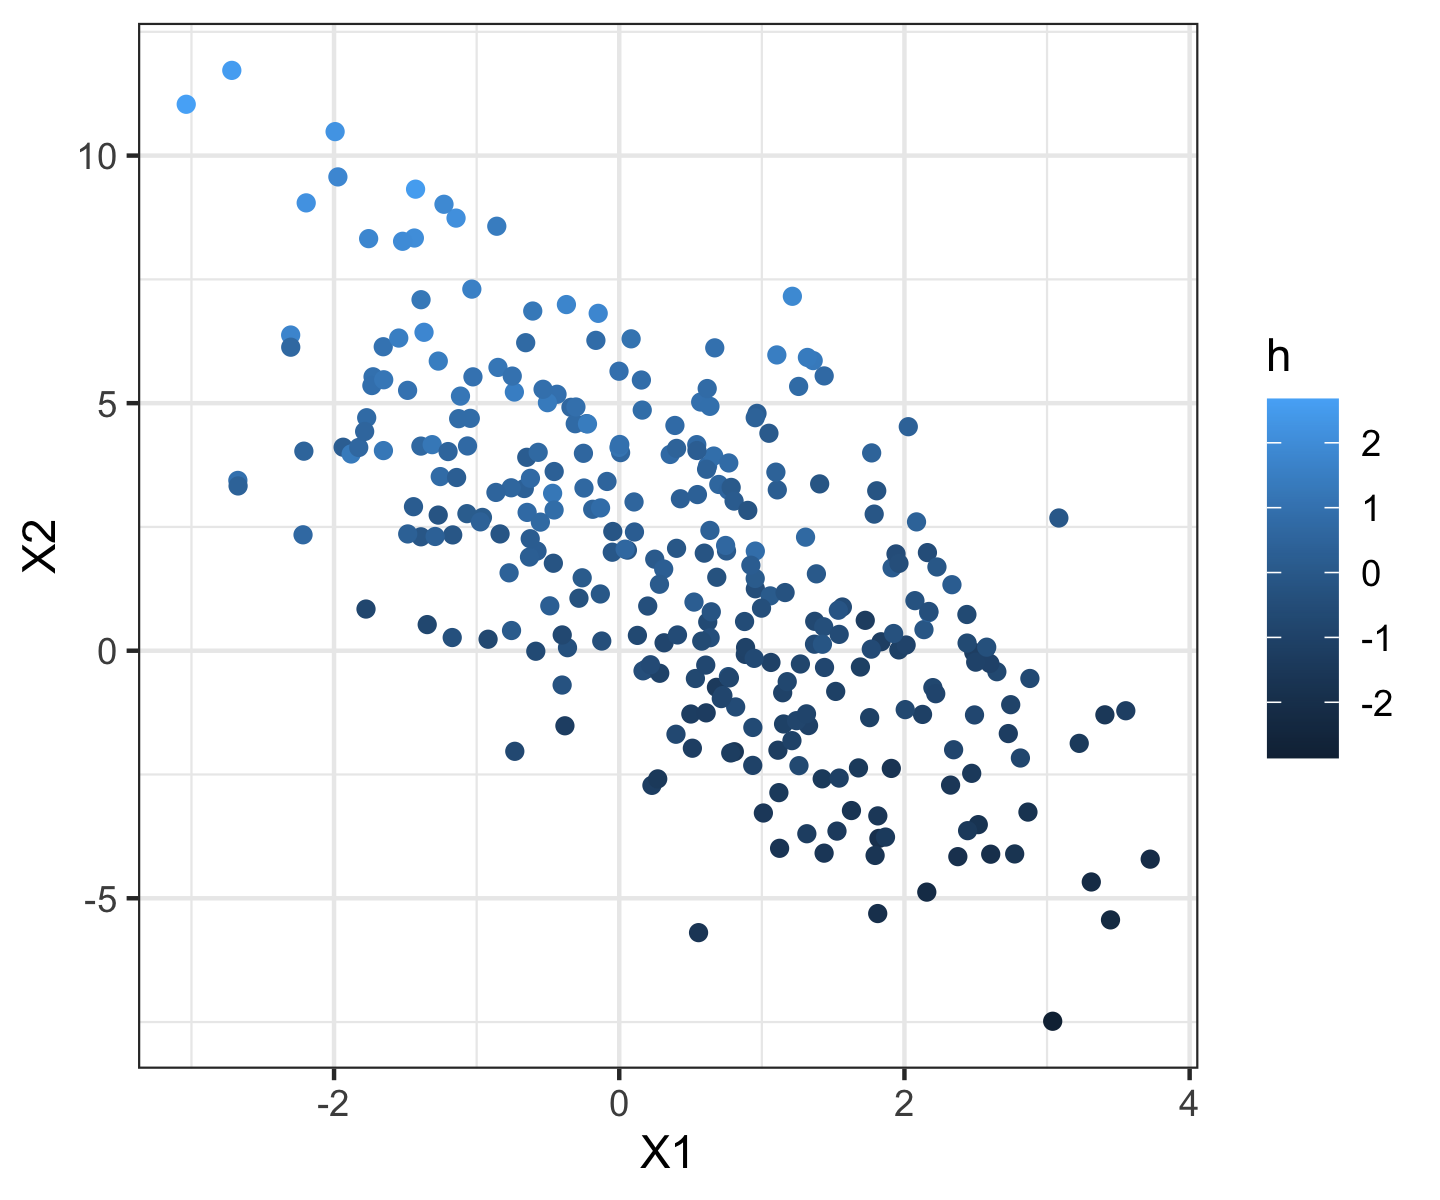
\includegraphics[width=0.9\textwidth]{fig/pPCA_h.png}
\caption{Data from a pPCA model with $W = (-1, 3)^T$, $b = (0.5, 2)$ and $\sigma^2 = 1$}
\end{figure}

\end{frame}


\begin{frame}{probabilistic PCA}

\begin{itemize}
\item probabilistic PCA
\[
x_i = b +  W h_i^T + \epsilon_i
\]
\pause
\item We can now {\color{uured} estimate our parameters} using EM \\ (or Bayesian methods)
\item Enables us to {\color{uured} combine with other models} \\ (e.g. mixture of pPCA)
\pause
\item And as we will see next week, is the {\color{uured} basic building block} for many high-dimensional problems
\end{itemize}

\end{frame}


\begin{frame}{Connections to PCA and Factor Analysis}

\begin{itemize}
\item probabilistic PCA
\[
x_i = b +  W h_i^T + \epsilon_i
\]
where $\epsilon \sim N(\mathbf{0}, \Psi)$
\item pPCA is closely connected to PCA and Factor Analysis:
\begin{itemize}
\item $\sigma I \rightarrow 0$: pPCA $\rightarrow$ {\color{uured} PCA}
\item $\Psi = \text{diag}(\sigma_1, ..., \sigma_p, ..., \sigma_P)$: pPCA $\rightarrow$ {\color{uured} Factor Analysis}
\end{itemize}
\end{itemize}

\end{frame}


\end{document}
